\section{Problem Statement}
This project was created to solve the problem caused by feature extraction on large grids.
High resolution grids are blessed with precise and plentiful data, but cursed by large file sizes.
Extracting features on these requires millions of computations hundreds of computing hours.
However, these extracted features are absolutely required to produce accurate models.
\begin{figure}[h]
    \centering
    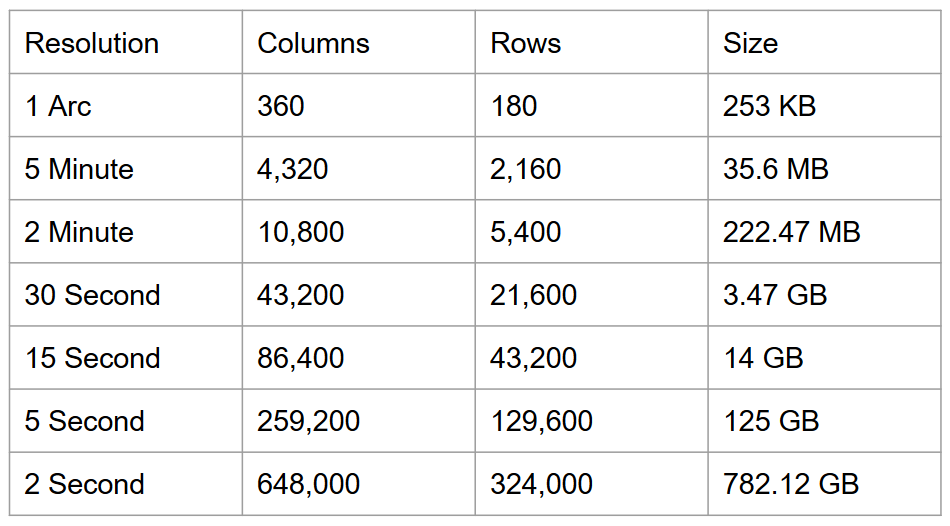
\includegraphics[scale=0.5]{grid_sizes}
    \caption{Graphic showing the sizes of grid files}
  \end{figure}

\par
Programs for extrating these features have been written. 
They were written with fortran, and ran in serial.
The preformance was sufficent for lower resolution grids, but this does not scale to larger grids.
Larger grids require hundreds of hours to complete.
Some statistics scale even worse.
Requiring potentially thousands of hours to compute. 
This leaves a need for quick quick computation.
The size of the grids is also a limiting factor. 
Some of the larger grids require hundreds of gigabytes to represent in memory.

\par
The time complexity for feature extraction effects the ability to test new statistics.
Being able to stream new statistics into models is an efficent way to determine the best features for an accurate model.
This is hindered by the computation time for feature extraction.
New features can not be tested in a model if they have not been computed.
Therefore, the computation bottle neck directly effects the ability to test new models essipically at higher resolutions.

\par
This project needs to solve the following problems.
We need to be able generate new statistics in a time prohibitive mannager.
We also need to create a way to implement new statistics for quick iterative testing with models.
It is also imperative that a solution for handling large grids on a variety of systems is developed.
This will allow our solution to scale up or down.

